\documentclass[10pt] {article}
\usepackage[portuguese]{babel}
\usepackage[utf8]{inputenc}
\usepackage{graphicx}
\usepackage[labelformat=empty]{caption}
\setcounter{secnumdepth}{5}
\setcounter{tocdepth}{5}

\usepackage{geometry} % Required to change the page size to A4
\geometry{a4paper} % Set the page size to be A4 as opposed to the default US Letter

\usepackage{indentfirst} %Identação nos parágrafos iniciais

% Code
\usepackage{listings}

\lstset{language=C, breaklines=true, basicstyle=\footnotesize} % Especificar Haskell, mudar de linha quando acabar espaço, diminuir tamanho da letra.

\usepackage{fixltx2e} % Corrige alguns erros


\begin{document}

\title{Relatório Trabalho Prático C \\ $\small{Grupo 13}$}

\maketitle

%--------------------------------
% Group Members
%--------------------------------
\begin{figure}[!htb]
\minipage{0.32\textwidth}
  
\includegraphics[width=\linewidth]{jc.jpg}
  \caption{João Costa A70563}\label{fig:awesome_image1}
\endminipage\hfill
\minipage{0.32\textwidth}
  
\includegraphics[width=\linewidth]{ls.jpg}
  \caption{Leandro Salgado A70949}\label{fig:awesome_image2}
\endminipage\hfill
\minipage{0.32\textwidth}%
  
\includegraphics[width=\linewidth]{ma.jpg}
  \caption{Martinho Aragão A72205}
\endminipage
\end{figure}

\newpage

\tableofcontents

\newpage

\section{Introdução}
\par Este relatório aborda a resolução do projeto prático em C de LI3. O Projeto, denominado Gesthiper, baseia-se
num programa de gestão de hipermercados o qual depende de uma lista de clientes, uma lista de produtos e uma
lista de compras efetuadas. \par Cada uma destas listas deve estar num ficheiro .txt e para cada um dos ficheiros o
programa percorre o ficheiro, executando operações que permitam guardar estes dados em memória. Para ajudar nesta tarefa repartiu-se as tarefas em quatro módulos
módulos. Estes módulos são: um catálogo de clientes; um catálogo de produtos; um módulo de contabilidade; e um módulo de compras.
\par De forma a preservar o encapsulamento de dados disponibilizou-se uma API de
forma a que o utilizador apenas possa aceder através destas funções públicas.
\par Depois dos ficheiros serem carregados o utilizador é capaz de executar uma lista de queries que
foi fornecida pela equipa docente. Para responder às diferentes queries utiliza-se as funções definidas nas API dos diferentes
módulos já referidos bem como código auxiliar presente no \emph{main}, programa principal.
\par Ao longo deste relatório aborda-se assim as decisões tomadas na implementação do projeto, nomeadamente quais as estruturas utilizadas para criar cada um dos módulos e as suas APIs.

\newpage
\section{Módulos}
Na seguinte seção apresentam-se desenhos comentados das estruturas de dados,
todos os typedef e a documentação da API comentada, função a função.

%------------------------
% Clients
%------------------------

\subsection{Catálogo Clientes}
\par Esta subsecção trata da API do catálogo de clientes e da sua implementação.

\subsubsection{Estrutura de Dados}
\par
Para guardar os clientes lidos a partir do ficheiro resolvemos usar uma Trie pois apesar de
necessitar de mais instruções a procura é igualmente rápida. A seguir fica um exemplo da Trie implementada,
cada nodo contêm um caracter e apontadores para próximo, anterior, pai e filhos.

\begin{figure}[ht!]
\centering
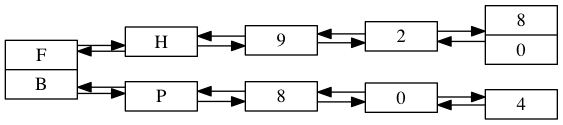
\includegraphics[width=70mm, height=20mm]{trie.png}
\caption{Trie com os clientes FH928, FH920 e BP804}
\end{figure}

\subsubsection{Definições de dados (Typedef)}

\noindent\textbf{clients.h}
\begin{lstlisting}
typedef struct node * ClientsCat; /* Catalogo de Clientes */
\end{lstlisting}
\textbf{clients.c}
\begin{lstlisting}
struct node {
  char value; /* Carater a guardar */
  struct node * next; /* Proximo nodo */
  struct node * prev; /* Nodo anterior */
  struct node * children; /* Nodo filho */
  struct node * parent; /* Nodo pai */
};
\end{lstlisting}
\par {O typedef no ficheiro \emph{clients.h} é a única informação que o utilizador têm relativamente à implementação
de dados, não tendo  acesso ao ficheiro .c dos clientes não consegue conhecer a verdadeira implementação da
estrutura \textbf{node}. Deste modo garantimos o encapsulamento de dados e a única forma do utilizador interagir
com o catálogo de clientes será através da API;} \\

\subsubsection{Funções API}

% initClients
\noindent\textbf{ClientsCat initClients()}
\par Inicializa a estrutura do catálogo de clientes.

% insertClient
\noindent\textbf{ClientsCat insertClient (ClientsCat cat, char * client)}
\par Insere um dado client, o argumento \emph{client}, na estrutura de clientes, argumento \emph{cat}.
\par Se a estrutura não tiver sido inicializada ou o cliente não existir a função retornou o valor \emph{NULL},
caso contrário devolve o valor cat, isto permite que duas variáveis trabalhem na mesma estrutura. \\

% searchClient
\noindent \textbf {Bool searchClient (char * client)}
\par Verifica se um cliente, o argumento \emph{client}, existe no catálogo de clientes.
\par A função devolve um valor do tipo Bool, definido em \emph{"Boolean.h"}, que será \emph{true} se o
cliente existir no catálogo e \emph{false} caso contrário. \\

% removeClient
\noindent \textbf{ClientsCat removeClient(ClientsCat cat, char * client)}
\par Remove um cliente, o argumento \emph{client}, de um dado catálogo de clientes, o argumento \emph{cat}.
\par A função retorna \emph{NULL} caso a estrutura não tenha sido inicializada ou o cliente seja inválido, e
retorna a própria estrutura caso contrário. \\

% searchClients
\noindent \textbf{StrList searchClients (ClientsCat cat, char init)}
\par Cria lista com todos os clientes cujo código comece por uma certa letra, o argumento \emph{init}, e que
estejam presentes no catálogo, \emph{cat}, passado como argumento.
\par Como o utilizador não conhece a definição do tipo \emph{StrList} apenas a main sabe como utilizar
o valor devolvido pela função. \\

% numOfClients
\noindent \textbf{int numOfClients (ClientsCat cat)}
\par Calcula o número de clientes presentes no catálogo, \emph{cat}, fornecido como argumento.
\par Como o utilizador não sabe como é que a estrutura de dados do catálogo está definida não consegue
calcular o número de clientes no catálogo sem recorrer a esta função. \\

% deleteCat
\noindent \textbf{ClientsCat deleteCat (ClientsCat cat)}
\par Liberta a memória ocupada pelo catálogo de clientes fornecido como argumento, \emph{cat}.
\par A função retorna NULL se a libertação de memória for bem sucedida. \\

% validateClient
\noindent \textbf{Bool validateClient (char * client)}
\par Verifica se um dado cliente, o argumento \emph{client}, é válido. Um cliente é válido se os dois primeiros
caracteres forem duas letras maiúsculas e os restantes três caracteres forem números.
\par A função retorn \emph{true} se o cliente for válido e \emph{false} se não o for.


%------------------------
% Products
%------------------------

\newpage
\subsection{Catálogo Produtos}
\par Esta subsecção trata da API do catálogo de produtos e da sua implementação.

\subsubsection{Estrutura de Dados}
\par
Para guardar os produtos lidos a partir do ficheiro resolvemos usar uma Trie pois apesar de necessitar de mais instruções a procura é igualmente rápida. A seguir fica um exemplo da Trie implementada, cada nodo contém um array, e cada posição de cada array aponta para outro array ou \emph{NULL}. Os caracteres são implicitamete definidos pela sua posição no array, e o código de produto é guardado no último nodo.


\begin{figure}[ht!]
\centering
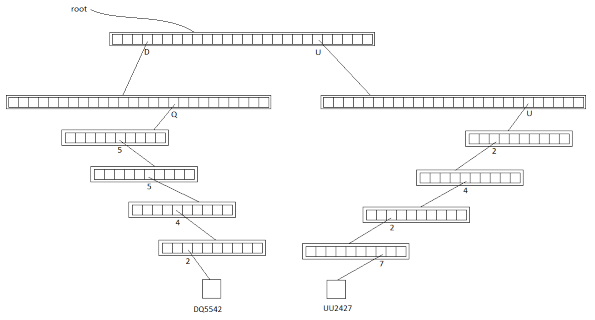
\includegraphics[width=80mm, height=50mm]{trie2.png}
\caption{Trie com os produtos DQ5542 e UU2427}
\end{figure}

\subsubsection{Definições de dados (Typedef)}

\noindent\textbf{products.h}
\begin{lstlisting}
typedef struct node ProductsCat; /* Catalogo de Produtos */
\end{lstlisting}
\textbf{products.c}
\begin{lstlisting}
struct node{
	int qnt; /* Valor que no primeiro nodo diz quantos produtos daquela inicial existem, e que  */no ultimo nodo marca o produto como comprado ou nao
	char code[6]; /*Codigo a guardar */
	struct node* link[ALPHA]; /*Array seguinte */
};
\end{lstlisting}
\emph{typedef struct node ProductsCat;} - Catálogo de Produtos
\par Este typedef é a única informação que o utilizador têm relativamente à implementação de dados, não tendo
acesso ao ficheiro .c dos produtos não consegue conhecer a verdadeira implementação da estrutura \textbf{node}.
Deste modo garantimos o encapsulamento de dados e a única forma do utilizador interagir com o catálogo de
produtos será através da API;

\begin{lstlisting}
typedef struct listnode PList; /* Lista de Produtos */
\end{lstlisting}
\textbf{products.c}
\begin{lstlisting}
struct listnode{
	int qnt; /*Valor que diz quantos produtos estao no array de Strings */
	char **codes; /*Array de Strings que guarda codigos de Produtos */
};
\end{lstlisting}

\par Este typedef é referente a uma estrutura utilizada para guardar produtos. Uma vez que é desconhecido ao
utilizador como está definido o tipo \emph{struct listnode}, foram implementadas funções de acesso à estrutura
de modo a garantir o encapsulamento de dados.

\subsubsection{Funções API}

% initProductsCat
\noindent \textbf{ProductsCat* initProductsCat()}
\par Inicializa a estrutura do catálogo de produtos.

%insertProduct
\noindent \textbf{ProductsCat* insertProduct(ProductsCat *root, char key[])}
\par Insere um produto, argumento \emph{key}, na estrutura de produtos, argumento \emph{root}.
\par Se a estrutura de produtos não tiver sido inicializada, é inicializada, o produto é inserido na mesma e é retornado o valor de \emph{root}.
\par Caso o argumento \emph{key} seja inválido, isto é, se não for constituído por dois caracteres seguidos de quatro algarismos, é retornado o valor 0.

%searchProduct
\noindent \textbf{Bool searchProduct(ProductsCat *prodcat, char key[])0}
\par Procura um produto, argumento \emph{key}, na estrutura de produtos, argumento \emph{prodcat}.
\par Se a estrutura de produtos não tiver sido inicializada, é retornado \emph{false}.
\par Se o produto for encontrado, é retornado \emph{true}. Caso contrário, é retornado \emph{false}.

%search4Product
\noindent \textbf{Bool search4Product(ProductsCat *prodcat, char key[])}
\par Procura um produto, argumento \emph{key}, na estrutura de produtos, argumento \emph{prodcat}.
\par Se a estrutura de produtos não tiver sido inicializada, é retornado \emph{false}.
\par Se o produto for encontrado, o produto é marcado e é retornado \emph{true}. Esta marca será utilizada para saber se o produto foi comprado ou não. Caso o produto não seja encontrado, é retornado \emph{false}.

%searchI
\noindent \textbf{PList* searchI(ProductsCat *prodcat, char c)}
\par Procura na estrutura de produtos, argumento \emph{prodcat}, todos os produtos que seja começados por uma determinada letra, argumento \emph{c}.
\par Os produtos são guardados numa estrutura \emph{PList}, cujo valor será retornado.
\par A estrutura \emph{PList} não necessita de inicialização manual.

%productsNotBought
\noindent \textbf{PList* productsNotBought(ProductsCat *procat)}
\par Procura na estrutura de produtos, argumento \emph{prodcat}, todos os produtos que não tenham sido comprados, isto é, todos os produtos que não tenham sido marcados pela função \emph{search4Product}.
\par Os produtos são guardados numa estrutura \emph{PList}, cujo valor será retornado.
\par A estrutura \emph{PList} não necessita de inicialização manual.

%removeProduct
\noindent \textbf{ProductsCat* removeProduct(ProductsCat *prodcat, char key[])}
\par Remove um produto, argumento \emph{key}, da estrutura de produtos, argumento \emph{prodcat}.
\par A função devolve o valor \emph{prodcat}.

%deleteProductCatalog
\noindent \textbf{ProductsCat* deleteProductCatalog(ProductsCat *prodcat)}
\par Elimina o catálogo de produtos, argumento \emph{prodcat}, e liberta todo o espaço em memória ocupado pelo mesmo.
\par Devolve um \emph{NULL} do tipo \emph{ProductsCat}.

%numOfProducts
\noindent \textbf{int numOfProducts(ProductsCat *cat)}
\par Retorna o total de produtos da estrutura de produtos, argumento \emph{cat}, que nunca foram comprados.

%getCode
\noindent \textbf{char* getCode(PList *p, int n)}
\par Função auxiliar de acesso à estrutura \emph{PList}.
\par Recebe a estrutura \emph{PList}, argumento \emph{p}, e um índice, argumento \emph{n}.
\par Devolve o código do produto presente na estrutura \emph{PList} cujo indice seja \emph{n}.

%getQnt
\noindent \textbf{int getQnt(PList *p)}
\par Função auxiliar de acesso à estrutura \emph{PList}.
\par Recebe a estrutura \emph{PList}, argumento \emph{p}.
\par Devolve o número de códigos de produtos na estrutura \emph{PList}.

%freeList
\noindent \textbf{void freeList(PList *p)}
\par Função que liberta todo o espaço ocupado pela estrutura \emph{PList}, argumento \emph{p}.


%------------------------
% Accounting
%------------------------

\newpage
\subsection{Contabilidade}
\par Esta subsecção trata da API do módulo de Contabilidade da sua implementação

\subsubsection{Estrutura de Dados}
\par
Para guardar informação relativa à contabilidade, resolvemos usar um array de 12 AVLs pois esta estrutura permite ordenar estruturas complexas de acordo com um método de comparação, separando pelos 12 meses. Como nesta situação existe ordem alfabética segundo o código de produto, então uma AVL permite fazer procura rápida (comparação de strings), preservando mesmo assim memória.

\subsubsection{Definições de dados (Typedef)}

\begin{lstlisting}
typedef struct treeNode{
  char code[6];
  int normalNumber;
  double normalMoney;
  int promotionNumber;
  double promotionMoney;
  int height;
  struct treeNode *left;
  struct treeNode *right;
} ProductNode;
\end{lstlisting}

\par AVL com informação do número de vendas e seu valor distinguido por normal ou promoção, ordenada pelo código do produto, e com informação adicional sobre a altura do nodo na árvore. Para encapsulamento, encontra-se no .c .

\begin{lstlisting}
typedef struct {
  struct treeNode * monthAccounting[12];
  int sales[12];
} Accounting;
\end{lstlisting}
\begin{figure}[ht!]
\centering
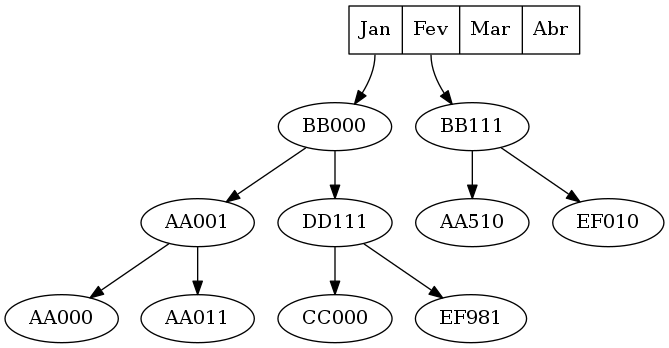
\includegraphics[width=80mm]{accounting.png}
\caption{Array de 12 AVLs, distribuição por meses.}
\end{figure}

\subsubsection{Funções API}
\noindent \textbf {Accounting * initAccounting()}
\par Inicializa a estrutura de contabilidade.  Para garantir o encapsulamento de dados a função devolve um valor do tipo \emph{Accounting *} o qual o utilizador da API
não tem conhecimento de como está definido pois não conhece a \emph{struct treeNode.} \\

\noindent \textbf {Accounting * insertAccounting(Accounting *, Tokens *)}
\par Insere a informação da venda de um dado produto \emph{Tokens *}, no argumento \emph{Accounting *}, adicionando ou atualizando na árvore do respetivo mês.
\par Se a estrutura não tiver sido inicializada ou o cliente não existir a função retorna o valor \emph{NULL},
caso contrário devolve a estrutura atualizada. \\

\noindent \textbf {int removeAccounting(Accounting *, char *)}
\par Remove um produto da Contabilidade, o argumento \emph{char *} identifica o código do produto no array de árvores \emph{Accounting *}.
\par A função retorna \emph{NULL} caso a estrutura não tenha sido inicializada ou o cliente seja inválido, e retorna a própria estrutura alterada caso contrário. \\

\noindent \textbf {Bool searchAccounting(Accounting *, char *)}
\par Procura o código \emph{char *} de um produto, na Contabilidade \emph{Acccounting *}, passado como argumento. Retorna 1 caso encontre, e 0 caso contrário.
\par O encapsulamento é preservado pois o utilizador desconhece a implementação de \emph{treeNode}. \\

\noindent \textbf {OverallSales * getMonthlyProductSales(Accounting *, int, char *)}
\par Procura o código \emph{char *} de um produto e, de acordo com o mês \emph{int}, devolve um conjunto de informações sobre as compras, unidades vendidas em regime normal ou promoção e montante total.
\par A estrutura devolvida é uma cópia com informação genérica de acordo com o pedido. Consiste simplesmente por 4 números relativos a compras.

\noindent \textbf {OverallSales * getSalesbyMonthPeriod(Accounting *, int, int)}
\par De acordo com um período mensal de \emph{int} a \emph{int}, devolve o número de unidades vendidas e o rendimento total.
\par Utiliza mais uma vez a estrutura genérica de output de informação de contabilidade \emph{OverallSales}.

\noindent \textbf {void freeAccounting (Accounting *)}
\par Limpa uma estrutura \emph{Accounting *}, fazendo free das 12 árvores do array.

%------------------------
% Sales
%------------------------
\newpage
\subsection{Módulos Compras}

%-----------------------------
%	Sales by Products
%-----------------------------
\subsubsection{Compras ordenadas por códigos de produto}
\paragraph{Estrutura de Dados}
\indent\par Para organizar as compras por código de produto decidimos usar uma AVL em que os nodos
contém o código de produto, o número de quantidades compradas, o número de clientes que comprou
esse produto e um apontador para uma árvore AVL, na qual os nodos contém os códigos dos clientes que
compraram o produto e, para cada cliente, se a compra foi normal, em promoção ou ambas.

\begin{figure}[ht!]
\centering
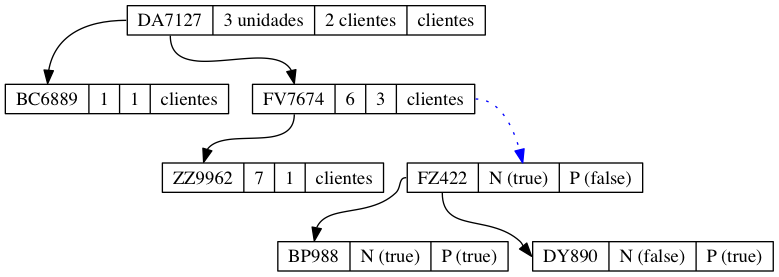
\includegraphics[width=100mm]{avl_salesp.png}
\caption{AVL com produtos, os clientes FZ422, BP988 e DY890 compraram o produto FV7674}
\end{figure}

 \paragraph {Definições de Dados (Typedef)}\mbox{}\\
 \textbf{salesp.h}
 \begin{lstlisting}
 typedef struct productNode * SalesP; /* AVL organizada por codigos de produto */
 typedef struct q12struct { /* Estrutura para a query 12 */
  StrList list; /* LIsta para guardar os produtos */
  int * quants; /* Array de quantidades */
  int * clients;  /* Array de numero de clientes */
} * topNP;
typedef struct topNP * q12struct; /* typedef para a query 12 */

 \end{lstlisting}
 \textbf{salesp.c}
 \begin{lstlisting}
 typedef struct clientNode {
  char client[6]; /* Codigo do cliente */
  Bool n; /* Compra normal */
  Bool p; /* Compra promocional */
  int height; /* Altura do nodo */
  struct clientNode * left, * right; /* Sub-arvores */
} ClientNode;

typedef struct productNode {
  char product[7]; /* Codigo do produto */
  int quant; /* Quantidade comprada */
  int qclients; /* Numero de clientes que compraram */
  int height; /* Altura do nodo */
  struct clientNode * clients; /* AVL com clientes que compraram o produto */
  struct productNode * left, * right; /* Sub-arvores */
} ProductNode;
\end{lstlisting}

 \par O utilizador apenas tem acesso aos \emph{typedef} nos ficheiro .h e portanto não tem ideia como está
 definida a estrutura \textbf{clientNode} ou \textbf{productNode}, assim sendo, a única maneira de interagir com o
 módulo de compras é através das funções disponibilizadas na API.

\paragraph{API AVL de Produtos}\mbox{}\\
\textbf {SalesP InitSalesP ()}
 \par Inicializa a AVL organizada por código de produtos, devolvendo o nodo do tipo \emph{SalesC}.
 \par O utilizador apenas sabe que está a ser utilizada uma árvore AVL, não sabendo como está definido o tipo
 \emph{SalesP} nem o tipo \emph{productNode} não tem como aceder as variáveis sem ser através das funções
 disponibilizadas pela API. \\

% insertProductSP
\noindent \textbf {SalesP insertProductSP (SalesP sales, char * product, int quant)}
\par Insere um produto, argumento \emph{product}, na AVL, e uma determinada quantidade \emph{quant},
devolvendo a AVL, é necessário guardar este valor pois a árvore pode sofrer rotações e não guardando o valor
provocará erros em futuras utilizações das funções. Caso o produto exista na AVL a sua quantidade é atualizada.\\

% insertClientSP
\noindent \textbf {SalesP insertClientSP (SalesP sales, char * product, char * client, char type)}
\par Insere um cliente, \emph{client}, na AVL de clientes que compraram o produto, \emph{product}, guardando
também informação sobre se a compra foi normal, \emph{type} com valor 0, ou compra em promoção,
\emph{type} com valor 1.\\

% clientsThatBought
\noindent \textbf {StrList clientsThatBought (SalesP sales, char * product)}
\par Cria uma lista com os clientes que compraram um determinado produto, \emph{product}, caso este exista em
\emph{sales}.\\

% topNProducts
\noindent \textbf {topNP topNProducts (SalesP sales, int n)}
\par Devolve uma variável do tipo \emph{topNP} com códigos de produtos, quantidades compradas e número de
clientes que compraram os produtos, para os \emph{n} produtos mais comprados durante o ano.\\

% freeSalesP
\noindent \textbf {void freeSalesP (SalesP sales)}
\par Apaga toda AVL \emph{sales} libertando assim a memória utilizada por este módulo de compras.\\

%-----------------------------
%	Sales by Clients
%----------------------------
\newpage
\subsubsection{Compras ordenadas por códigos de cliente}
\paragraph{Estrutura de Dados}\mbox{}\\
\indent\par Para ordenar as compras por código de cliente decidimos usar uma AVL na qual os nodos contem
o código de cliente e um array com 12 posições, meses, de apontadores para árvores em que os nodos
contem o codigo de produto.

\begin{figure}[ht!]
\centering
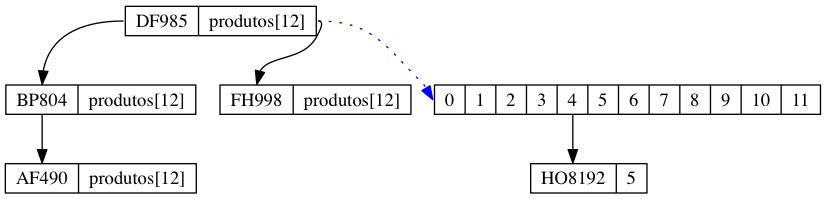
\includegraphics[width=120mm]{avl_salesc.png}
\caption{AVL com clientes, o cliente DF985 comprou 5 unidades do produto HO8192 em Maio}
\end{figure}

\paragraph{Definições de Dados (Typedef)}\mbox{}\\
\noindent\textbf{salesc.h}
\begin{lstlisting}
typedef struct clientNode * SalesC; /* AVL organizada por codigos de cliente */
\end{lstlisting}
\textbf{salesc.c}
\begin{lstlisting}
typedef struct productNode {
  char product[7]; /* Codigo do produto */
  int quant; /* Quantidade comprada */
  int height; /* Altura do nodo */
  struct productNode * left, * right; /* Sub-arvores */
} ProductNode;

typedef struct clientNode {
  char client[6]; /* Codigo de cliente */
  struct productNode * products[12]; /* AVL de produtos comprados pelo cliente */
  int height; /* Altura do nodo */
  struct clientNode *left, * right; /* Sub-arvores */
} ClientNode;
\end{lstlisting}

\paragraph{API AVL de Clientes}\mbox{}\\
 % initSales
\noindent \textbf {SalesC InitSales ()}
\par Inicializa a AVL organizada por código de clientes, devolvendo o nodo do tipo \emph{SalesC}.

% insertClientSC
\noindent \textbf {SalesC insertClientSC (SalesC sales, char * client)}
\par Insere um cliente, argumento \emph{client}, na AVL, devolvendo a AVL, é necessário guardar este valor
pois a árvore pode sofrer rotações e não guardando o valor provocará erros em futuras utilizações das funções. \\

%removeClientSC
\noindent \textbf {SalesC removeClientSC (SalesC sales, char * client)}
\par Remove um cliente, argumento \emph{client}, da AVL, argumento \emph{sales}. A função retorna a nova AVL
sem o nodo de cliente que foi especificado. \\

%insertProductSC
\noindent \textbf {SalesC insertProductSC (SalesC sales, char * client, \\ char * product, int month, int quant)}
\par Insere um produto, \emph{product}, como comprado pelo cliente, \emph{client}, num dado mês, \emph{month},
guardando também a quantidade comprada. Se o produto já existir a quantidade é atualizada. \\

%yearlyClients
\noindent \textbf {StrList yearlyClients (SalesC sales, StrList list)}
\par Cria uma lista com os códigos de clientes, presentes em \emph{sales}, que compraram produtos todos os
meses do ano, guardando numa lista passada como argumento, \emph{list}. \\

%clientMonthlySales
\noindent \textbf {ProductsN clientMonthlySales (SalesC sales, char * client)}
\par Calcula a quantidade de compras de um cliente \emph{client} por mês registadas em \emph{sales}. Retorna um array \emph{ProductsN} dos 12 valores.

%productsOnMonth
\noindent \textbf {StrList productsOnMonth (SalesC sales, char * client, int month)}
\par Cria uma lista com os produtos comprados por um dado cliente, \emph{client}, num dado mês, \emph{month},
caso o cliente esteja presente em \emph{sales}. \\

%topProducts
\noindent \textbf {StrList topProducts (SalesC sales, char * client)}
\par Cria uma lista com os três produtos mais comprados por um dado cliente, \emph{client}, caso esse cliente
esteja presente em \emph{sales}. \\

%clientMonthlyPurchases
\noindent \textbf {ClientsMonth clientsMonthlyPurchases (SalesC sales)}
\par Cria uma lista do número de clientes que realizaram compras por mês de acordo com a informação em \emph{sales}.
\par Retorna um array genérico com esses 12 valores de forma a preservar o encapsulamento.

%freeSales
\noindent \textbf {void freeSales (SalesC sales)}
\par Apaga a AVL passada como argumento \emph{sales}, libertando toda a memória usada pela mesma. \\

\newpage
\section{Includes}
\par De forma a não só facilitar o trabalho mas também a ajudar na legibilidade do código criamos alguns .h
com tipos que facilitassem o desenvolvimento do projeto e que vamos aqui mencionar.

\textbf{bool.h}
\begin{lstlisting}
typedef enum { false, true } Bool; /* Para definir o tipo booleano */
\end{lstlisting}

\textbf{max.h}
\begin{lstlisting}
#define MAX(A,B) ((A > B) ? A : B) /* Para calcular o maximo */
\end{lstlisting}

\textbf{overallsales.h}
\begin{lstlisting}
typedef struct {
  /* Calculates how many sales */
  int numberSales;
  /* Number of normal sales */
  int normalNumber;
  /* Number of sales in promotion */
  int promotionNumber;
  /* Total income */
  double income;
} OverallSales;
\end{lstlisting}

\textbf{salesstruct.h}
\begin{lstlisting}
/* Pointer to an array of ints by month */
typedef struct ProductsNStruct{
  int productsBought[12];
} * ProductsN;

/* Pointer to an array of ints by month */
typedef struct ClientsMonthStruct{
  int number[12];
} * ClientsMonth;
\end{lstlisting}

\textbf{StrList.h}
\begin{lstlisting}
typedef struct strlist { /* Lista de strings */
  char * clients[200000]; /* Apontados para strings de clientes/produtos */
  int size; /* Numero de strings presentes */
} * StrList;
\end{lstlisting}

%gesthiper.c
\newpage
\section{Main}
\par O programa principal resume-me a um conjunto de funções auxiliares de forma a simplificar a revisão do código.

\begin{description}
  \item[Menu] Uma função que imprime o menu ao utilizador, recebendo a opção.

  \item[Carregar Catálogo Clientes] Lê um ficheiro dado pelo utilizador e carrega o catálogo de clientes.

  \item[Carregar Catálogo Produtos] Lê um ficheiro dado pelo utilizador e carrega o catálogo de produtos.

  \item[Funções de validação] As funções \emph{trimSale} e \emph{validateSale} que validam uma linha de compras.

  \item[Carregar Compras] Lê um ficheiro de compars e carrega o módulo de compras e contabilidade.

  \item[Queries] Uma função para cada query a partir da 4.

  \item[Main] Carrega cada um dos módulos com um nome default de ficheiro. Tem um ciclo que só termina de acordo com as opções escritas pelo utilizador, com um switch que chama as funções para cada uma das queries, bem como para a alteração de ficheros.

\end{description}

% UI
\newpage
\section{Interface Utilizador}
\par Para ser possível realizar as queries foi necessário criar um menu inicial que não é mais que uma lista
com opções numeradas e cada opção tem a sua descrição, a partir deste menu inicial o utilizador apenas
tem que introduzir o número da opção que deseja aceder.
\par Para algumas das queries listas de \emph{Strings} têm de ser apresentadas, essas listas podem variar
muito  em tamanho e então era necessário uma maneira de as apresentar no ecrã, sem sacrificar a leitura das
mesmas.
\par Para apresentar as listas foi criado uma estrutura \emph{StrList} que contêm um array de {* char} e um campo
com o número de \emph{Strings} guardadas. Decidimos mostrar 20 linhas e 3 colunas de \emph{Strings},
dando um total de 60 \emph{Strings} no ecrã ao mesmo tempo, este número faz com que seja fácil visualizar a lista
quando o terminal ocupa 1/4 do ecrã. As \emph{Strings} são então dividas por páginas e o número de página
atual e o número total de páginas é apresentado no ecrã.
\par Foi também criado um menu quer permite ao utilizador navegar nas páginas, especificando se quer ir para a
próxima página, para a página anterior ,para uma página especifica ou então voltar ao menu inicial.
\par Quando o utilizador decide voltar ao menu a função `displayList' liberta todo o espaço em memória utilizado
pela lista que está a apresentar libertando todas as \emph{Strings} alocadas na lista e no fim libertando a propria
estrutura.
\par Também há queries que requerem a apresentação de tabelas, para cada uma dessas queries existe uma
função especializada que trata de apresentar a tabela no terminal do utilizador, contudo a navegação na é
igual relativamente às listas, os dados são dividos em páginas e as opções de navegação são as mesmas. O único
aspeto diferente é a apresentação em que cada dado é apresentado na sua própria linha e apenas são
apresentados 20 resultados de cada vez.

\newpage
\section{Makefile e Gráfico de Dependências}
\indent\par De seguida é apresentada a Makefile, e o gráfico de dependências gerado a partir da Makefile.
\begin{figure}[ht!]
\centering
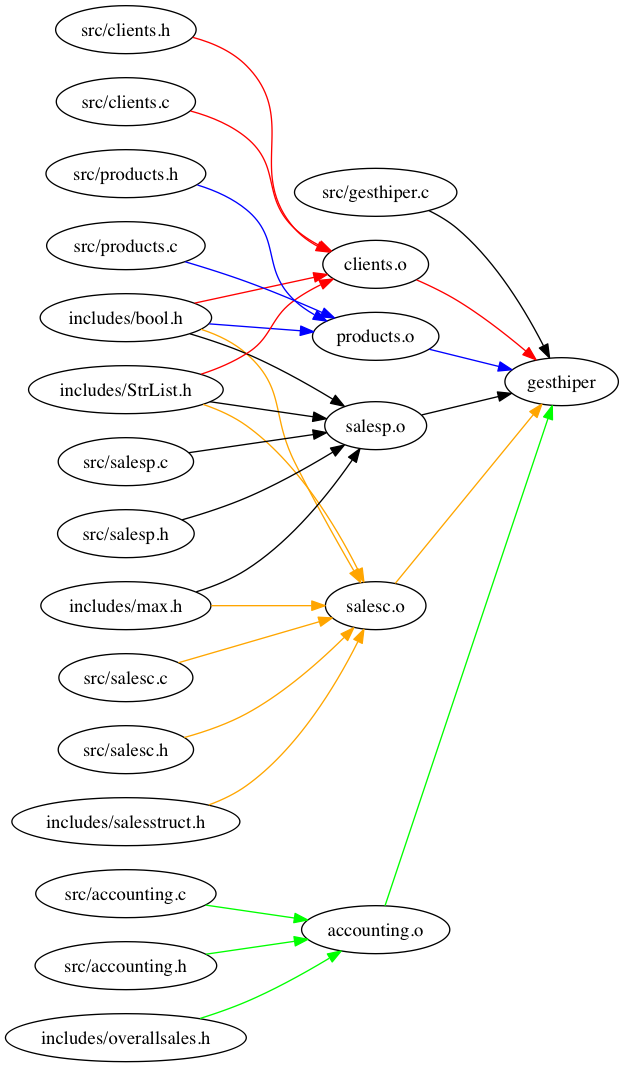
\includegraphics[height=120mm, width=80mm]{dep_graph.png}
\caption{Gráfico de dependências, gerado a partir da Makefile}
\end{figure}
\par O gráfico foi gerado a partir da Makefile:
\begin{lstlisting}
CFLAGS=-Wall -ansi -pedantic -O2

gesthiper: src/gesthiper.c clients.o products.o accounting.o salesc.o salesp.o
  gcc src/gesthiper.c clients.o products.o accounting.o salesc.o salesp.o
  $(CFLAGS) -o gesthiper -lm

clients.o: src/clients.c src/clients.h includes/bool.h includes/StrList.h
  gcc src/clients.c -c $(CFLAGS)

products.o: src/products.c src/products.h includes/bool.h
  gcc src/products.c -c $(CFLAGS)

accounting.o: src/accounting.c src/accounting.h includes/overallsales.h
  gcc src/accounting.c -c $(CFLAGS)

salesc.o: src/salesc.c src/salesc.h includes/bool.h includes/max.h
includes/salesstruct.h includes/StrList.h
  gcc src/salesc.c -c $(CFLAGS)

salesp.o: src/salesp.c src/salesp.h includes/bool.h includes/StrList.h
includes/max.h
  gcc src/salesp.c -c $(CFLAGS)
\end{lstlisting}

\newpage
\section{Conclusão}

\indent\par Em suma, apesar de cada uma das queries ter sido concluída, o trabalho mantém-se inacabado. De
facto, existem inúmeros pormenores que não foram resolvidos da melhor forma, como por exemplo a
eficácia da \emph{query 12}. Mesmo assim, a execução por módulos, com encapsulamento e abstração de dados
foi conseguida. Nota-se, no entanto, uma clara distinção entre a organização e o código dos diferentes módulos.
Outro dos problemas presentes, embora menor, é a não adoção das regras de C no que toca à designação de
nomes de variáveis e funções.
\par A grande conclusão a retirar deste trabalho prático é que quando se trabalha com vista responder a tantas
queries haverá sempre uma decisão a fazer, ou se perde mais tempo na inicialização do programa e se gasta
menos tempo na execução da tarefa ou, pelo contrário, se gasta menos tempo na inicialização e mais tempo na
execução da tarefa. Seja qual for a decisão tomada há sempre um sacrifício a fazer.
\par Em jeito de esclarecimento, o trabalho foi realizado em inglês por uma questão de aprendizagem no que toca à
utilização de ferramentas de código aberto, neste caso git através do GitHub. Deixou-se, no entando o STDIN e
STDOUT em português, pois o utilizador seria nesta língua.

\end{document}
